

\chapter{Material and methods}

%  Everything that is mentioned in results, has to be mentioned here
%  Everybody who reads thesis, must be able to reproduce the experiment/study
% o Describe all materials, devices and methods, which were used in your work
% o if you describe a device, start with the brand name followed by the company name, city and country in parentheses: e.g. "... a VersaHD (Elekta AB, Stockholm, Sweden) was used in ...".
% o Provide some information on each device
%  e.g Linac, which energies were used, what was the field size, what was the leaf width, how is the linac calibrated, ...;
%  e.g. Detector array: which type of detector, how many detectors, what is the resolution, energy dependence, linearity,...;
%  e.g. Panning systems: software version, algorithms, settings used in this study
%  e.g. software: version, functionality
% o Also describe used data (patient cohort) even if they were taken from other studies

\section{Scanners}

CT and MRI scanners used during this work are listed in Table \ref{tab:scanners}.

\begin{table}[h]
\centering
\begin{tabular}{llll}
System	& product name	& company	& coil [internal W x H]		\\
\toprule
MRI	& Magnetom C!	& Siemens	& Body/Spine Array Coil XL	\\
	&		&		& [50 x 30.5 cm (19.7 x 12 in)]	\\
CT	&		&		& --------
\end{tabular}
\caption{used scanners}
\label{tab:scanners}
\end{table}

\section{Custom build phantom}

To measure distortion the scanners must image a rigid object with known dimensions.
Such phantoms are commercially available, but often expensive and designed for a specific calibration protocol.
Some institutions build their own to fullfill exactly the requirements of a given application.

For the AKH it was important to create a lightweight phantom which can be imaged by CT and MRI scanners.
Due to the underlying physics, only fluids are visible in MRI scans. CT however, also shows plastic.
See figure \ref{fig:sagittal_comparison} for a comparison (MRI/CT visibility).
Therefore, they decided on plastic rods with a suitable fluid filling.
Such a liquid should be easily produced, non-toxic, and yielding sufficient signal in MRI scans.

Commercially available phantoms often resemble water filled tanks containing plastic grids as a reference.
This design results in stronger signal, but exceeds practical weight.
There are few brands offering solutions utilising liquid fiducial markers in the shape of pellets.
They are arranged in a regular pattern surrounded by air or plastic.
The AKH's design however relies on replaceable rods, which makes it a novelty.


\begin{figure}[!htb]
\centering
  \begin{subfigure}[b]{0.1\textwidth}
    
\includegraphics[scale=1]{slicer3D/full_phantom/sagittal_comparison_mr.png}
    \caption{MR}
    \label{fig:sagittal_comparison_mr}
  \end{subfigure}
  \begin{subfigure}[b]{0.1\textwidth}
    
\includegraphics[scale=1]{slicer3D/full_phantom/sagittal_comparison_ct_empty.png}
    \caption{CT}
    \label{fig:sagittal_comparison_ct_empty}
  \end{subfigure}
  \begin{subfigure}[b]{0.1\textwidth}
    
\includegraphics[scale=1]{slicer3D/full_phantom/sagittal_comparison_ct.png}
    \caption{CT}
    \label{fig:sagittal_comparison_ct}
  \end{subfigure}
  \caption{Comparison: MRI only shows liquid filling, CT also the plastic rod and pane (horizontal black bar crossing middle and right rod);\\ (\textbf{a:}) \textit{MRI} - filled rod, plastic not visible (field of view too small to show entire rod); (\textbf{b:}) \textit{CT} - empty rod, plastic visible; (\textbf{c:}) \textit{CT} - filled rod, plastic and filling visible}
  \label{fig:sagittal_comparison}
\end{figure}

\subsection{Frame and rods}

For the open-bore MRI scanner the phantom was build to fit exactly the scanner's coil.
Three parallel acrylic glass panes in the shape of the coil serve as a rigid frame.
In the middle an empty area was reserved for an optional additional smaller phantom (not used for this work).
Figure \ref{fig:phantom_photo} shows an picture of the phantom. See also figure \ref{fig:axial_CT_pane} showing a CT image of one pane (with no rods inserted). \\
More than 300 plastic rods (length: 50cm, outer diameter: 8mm, inner diameter: 4mm, volume: approx. 6mL) could be placed in the phantom.
See figure \ref{fig:rod_schematic} for a schematic sketch.
The bottom part of each rod was sealed with a hot glued plastic plug, the top could be closed with a plastic screw.
Frame and rods were already build and assembled before the author started working on this project.


% photo of phantom

\begin{figure}[!tbp]
\centering
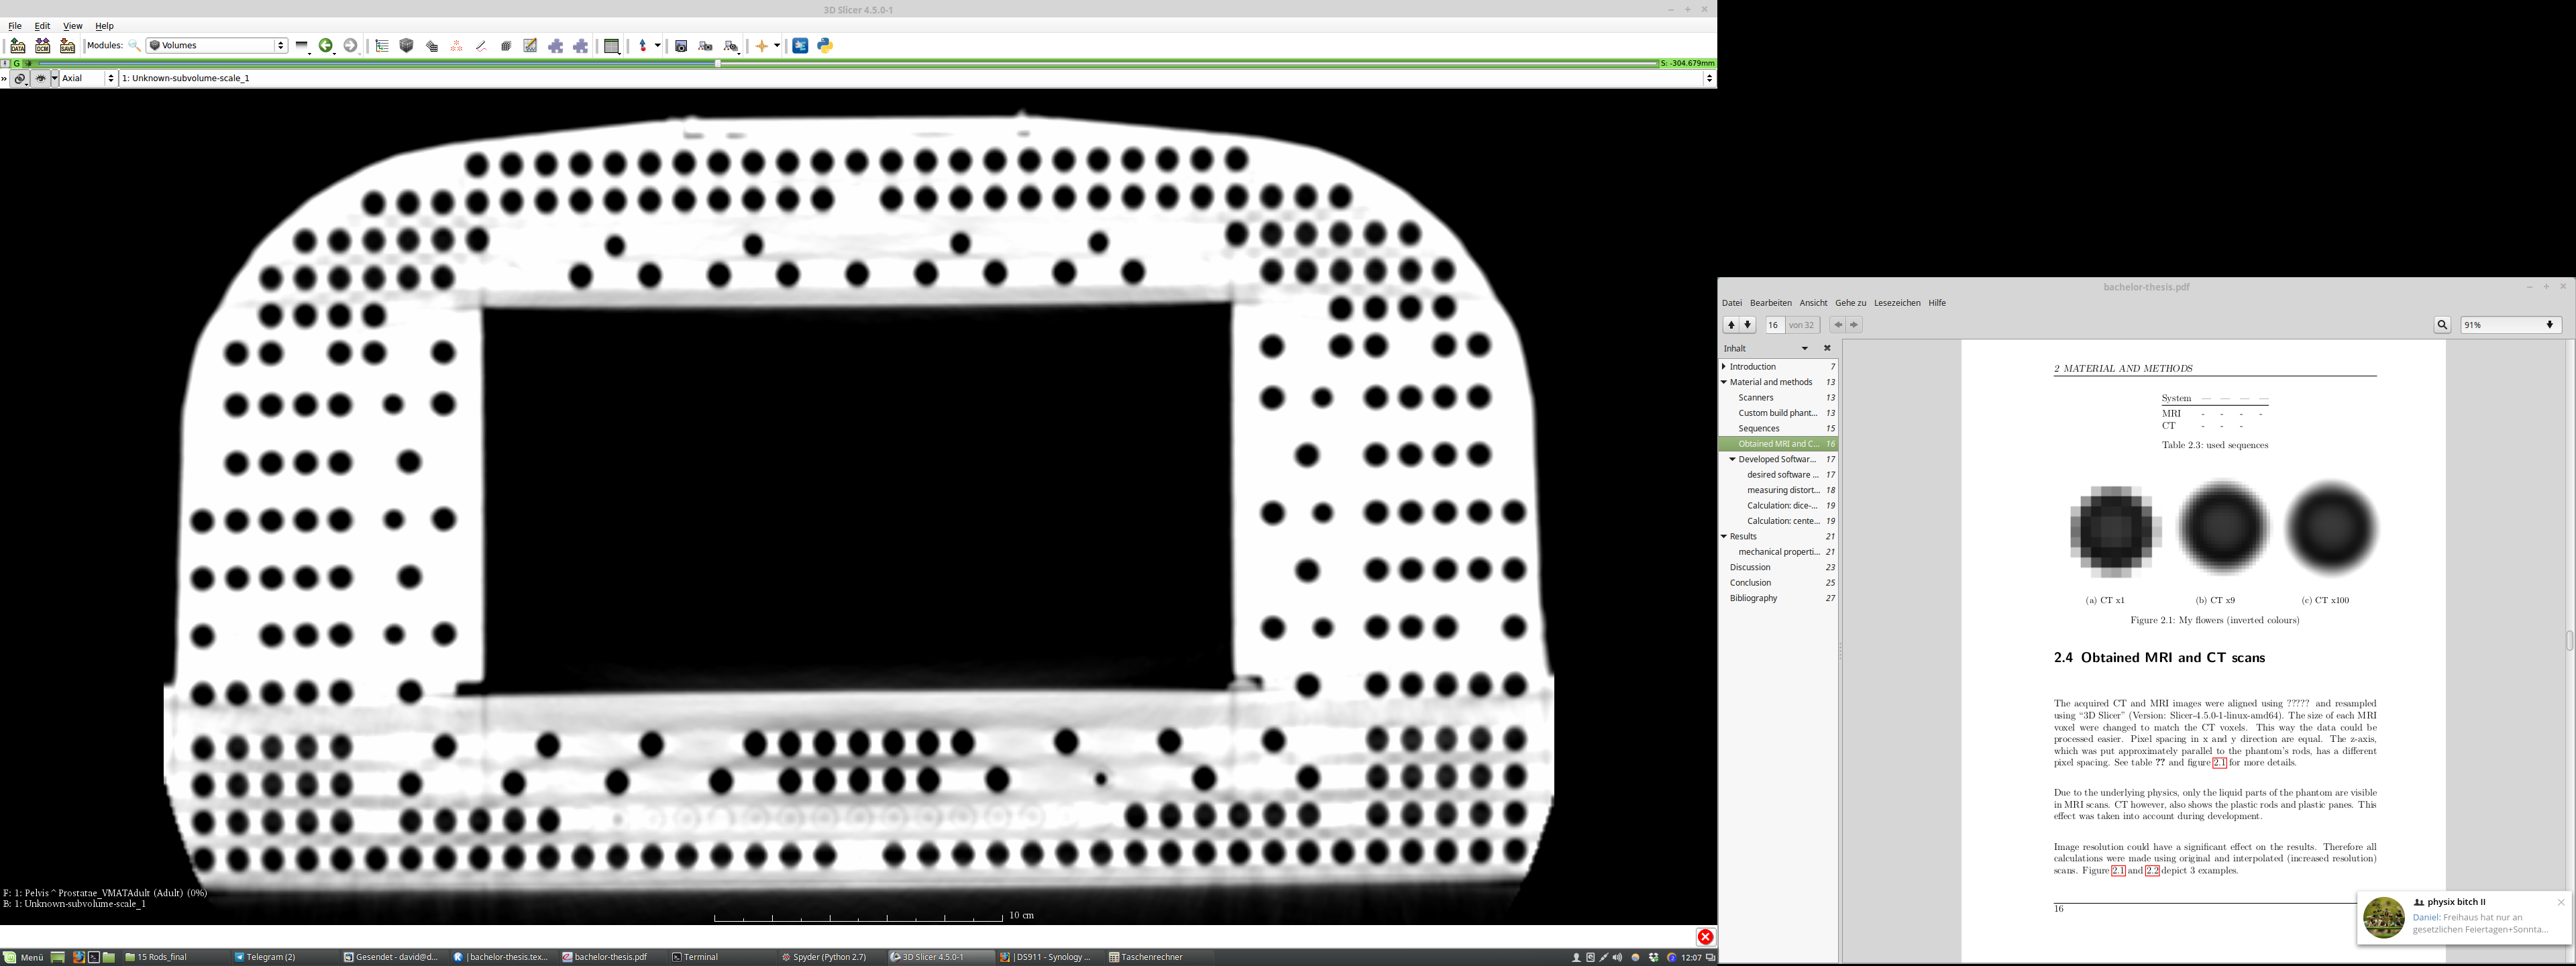
\includegraphics[width=\textwidth]{slicer3D/full_phantom/axial_CT_pane.png}
\caption{plastic pane, no rods inserted}
\label{fig:axial_CT_pane}
\end{figure}

\begin{figure}[!tbp]
\centering
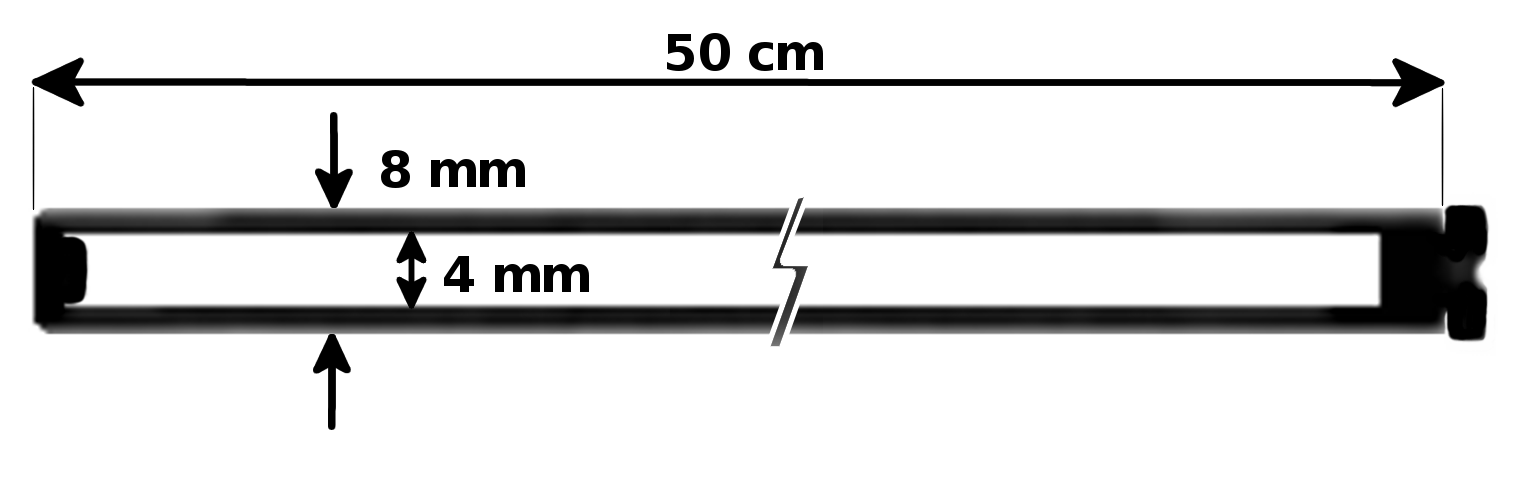
\includegraphics[width=0.8\textwidth]{slicer3D/full_phantom/rod_schematic.png}
\caption{empty plastic rod, schematic (not true proportions); }
\label{fig:rod_schematic}
\end{figure}

\vspace{4cm}
\textit{photo of Phantom}
\vspace{2cm}
\vspace{4cm}
\textit{photo of single rod}
\vspace{2cm}

\subsection{Rod fillings}

For this study 17 different liquids were produced to be tested as possible fillings. They are listed in Table \ref{tab:solutions}.

Most tested fluids are based on water. This makes it easy to empty and clean the rods if needed. They could then be filled again with a different liquid.
The chosen components are either non-toxic or harmless if not swallowed.
Unfortunately the water might evaporate over time. To improve the mobility of trapped air bubbles, soap was added to some fluids.

As an alternative 2 oils were proposed. They do not contain water and air is not soluble in oil. Once a rod is completely with oil, no air bubbles should form.
Using vegetable oil would be a non-toxic solution. This has been ruled out as a filling, because it would eventually rot.
Mineral oil on the other hand does not rot.


\begin{table}[!hbt]
\centering
\begin{tabular}{@{}l|rrrrrr@{}}
Nr.   & $NaCl$   & $CuSO_4\cdot5H_2O$          & Soap & Ascorbic Acid & Agar & Primovist [volume-\%]\\
\toprule
\#1  &             &                   &      &               &           &		\\
\#2  & 3.6         & 1.96              &      &               &           &		\\
\#3  & 3.6         & 3.92              &      &               &           &		\\
\#4  & 3.6         & 19.6              &      &               &           &		\\
\#5  & 3.6         & 1.96              & 1    &               &           &		\\
\#6  & 3.6         & 1.96              & 5    &               &           &		\\
\#7  & 3.6         & 1.96              & 20   &               &           &		\\
\#8  & 3.6         & 1.96              &      & 0.36          &           &		\\
\#9  & 3.6         & 1.96              &      & 3.6           &           &		\\
\#10 & 3.6         & 1.96              &      & 36            &           &		\\
\#11 & 3.6         &                   &      &               &           & 0.1\%	\\
\#12 & 3.6         &                   &      &               &           & 1\%		\\
\#13 & 3.6         &                   &      &               &           & 10\%	\\
\#14 & 3.6         & 1.96              &      &               &  0.5      &		\\
\#15 & 3.6         & 1.96              &      &               &   20      &		\\
\midrule
\#16 & \multicolumn{2}{r}{Motor Oil:}   & \multicolumn{4}{l}{\textit{Castrol Power1}}      \\
\#17 & \multicolumn{2}{r}{Silicon Oil:} & \multicolumn{4}{l}{\textit{Charge: 15HLVY023}}   \\ \bottomrule
\end{tabular}
\caption{composition of tested solutions\\(components in $g/L$; exception: Primovist in volume\%)}
\label{tab:solutions}
\end{table}

\newpage
\begin{enumerate}[label=\textbf{\#\arabic*}]
 \item \textit{destilled water} (as reference)
 \item $NaCl$ + $CuSO_4\cdot5H_2O$ (as suggested by AAPM MR Subcommittee \cite{Jackson2009})
 \item increased concentration of $CuSO_4\cdot5H_2O$
 \item further increased concentration of $CuSO_4\cdot5H_2O$
 \item generic washing-up \textit{soap} added to \textbf{\#2} (suggestion by Data Spectrum Corporation \cite{bubbles} to keep air bubbles from sticking to phantom walls)
 \item increased \textit{soap} concentration
 \item further increased \textit{soap} concentration
 \item \textit{ascorbic acid} added to \textbf{\#2} (reduce forming of air bubbles by binding dissolved oxygen. It then degrades to dehydro-ascorbic acid and water.
  \cite{Abtahi2008, Bodannes1979} Concentration of $0.36 \; g/L$ corresponds to approx. $0.00204 \; mol/L$)
 \item increased \textit{ascorbic acid} concentration
 \item further increased \textit{ascorbic acid} concentration
 \item \textit{Primovist} (a common contrast agent used for MRI scans \cite{VanBeers2012, Rohrer, primovist})
 \item increased amount of \textit{Primovist}
 \item further increased amount of \textit{Primovist}
 \item \textit{agar} (or agarose is commonly used as basic reference material for MRI phantoms \cite{BuccioliniCiraolo1989, Mathur-DeVre1985})
 \item increased \textit{agar} concentration
 \item synthetic motor oil
 \item silicon Oil
\end{enumerate}

% why those solutions??

Being closed at one end and having a capillary shape (small diameter) makes it impossible for the rods to be filled by pouring in the liquid.
Instead of adding the fluid at the top, it has to be injected starting at the bottom.
This way the contained air would pushed out through the opening on the top.
A thin plastic tube was used to leave room for the gas to escape.
Between different liquids the tube was flushed with \textbf{\#1} (distilled water) or \textbf{\#2} (main component of most solutions).

In order to minimize the amount of gas dissolved, the liquids were brought to boil shortly before injecting. Gas solubility generally decreases with rising temperature \cite{Henry1803, Sander2015}
After injecting the solution in the rods, they were left to cool down. Before closing the rods were topped up completely (no trapped air bubbles).
The oil based liquids, \textbf{\#16} and \textbf{\#17}, were not brought to boil.
Number \textbf{\#14} could be injected without problems, the solution remained fluid even after reaching room temperature.
Number \textbf{\#15} on the other hand changed to a gel like consistence and clogged the tube right after the rod was filled. The tube could not be used again.



\section{Sequences}

Following the suggestions given in the Report of AAPM MR Subcommittee TG1 ``MR Acceptance Testing and
Quality Control'' \cite{Jackson2009}, T1 weighted sequences were chosen to evaluate the possible solutions. (Table \ref{tab:settings})

\begin{table}[h]
\centering
\begin{tabular}{@{}lllll@{}}
System & ---  & --- &  --- & --- \\
\toprule
MRI    & -   & -   & -   & -    \\
CT     & -   & -   & -   &
\end{tabular}
\caption{used sequences}
\label{tab:settings}
\end{table}

\section{Developed software tool}

In order to asses the distortion of the MRI scanner, a tool was programmed.
It is written in Python 2.7 and uses the \textit{SimpleITK} package to read and process \textit{DICOM} (``\textit{Digital Imaging and Communications in Medicine}'') files. \cite{Python, DICOM}
\textit{SimpleITK} is a object-oriented ``C++ library with wrappers for Python, Java, CSharp, R, Tcl and Ruby''. \cite{SimpleITK, SimpleITK_started} It's versatility is one of the reasons why this approach was favoured.
It is a simplified layer built on top of the National Library of Medicine Insight Segmentation and Registration Toolkit (ITK). SimpleITK is also used by Applications like \textit{3D Slicer} , a ``free and open source software package for
visualization and medical image computing''. \cite{3DSlicer, Kikinis2012} For this work 3D Slicer was used to crop images, quickly read values and visualize the results.
Documentation and code examples of SimpleITK can be found at \cite{InsightSoftwareConsortium, Kyriakou-SimpleITK}
An alternative way to handle DICOM data in Python would be Pydicom. \cite{Pydicom, Kyriakou-Pydicom-VTK} 

An extensive list of packages used to process data:
\begin{itemize}
 \item SimpleITK
 \item numpy
 \item scipy
 \item matplotlib.pyplot \cite{Hunter2007}
 \item skimage.draw
 \item datetime
 \item os
\end{itemize}

\subsection{Processing MRI and CT scans}

% what application used to align CT and MRI
Prior to analising their data, the scans had to be prepared.
To start with, they were aligned in a way that yields maximum overlap especially in the centre of the image.
However, the MRI image had a lower resolution than the CT scan.
Therefore, the MRI voxel's size were changed to match the CT voxels. Both images were resampled to CT resolution.
Those steps were performed using \textit{MIRADA} (?????).

As described later, resolution might influence the efficiency of the distortion assesment.
The application \textit{3D Slicer} (Version: Slicer-4.5.0-1-linux-amd64) was used to again resample both images to a finer resolution.

Pixel spacing in x and y direction are equal. The z-axis, which lies approximately parallel to the phantom's rods, has a different pixel spacing.
Overall image resolution could have a significant effect on the results. Therefore all calculations were made using original and interpolated (increased resolution) scans.
See table \ref{tab:spacing} for more details. Figure \ref{fig:resample} depicts 3 CT/MRI scans of a single rod (axial) with different resolutions.
``x1'' stands for the original CT scan resolution (MRI resampled to match).
``x9'' is a resolution resulting in 1 pixel being splitted in 9 smaller pixels, ``x100'' in 100, and so on.
For better visibility images are printed with inverted colors. Dark pixels have a high density/intensity value, white pixels are equivalent to air (low density/intensity).

\begin{table}[!htb]
\centering
\begin{tabular}{l|l|l|l}
resample factor  & z (not affected) &  y (same as x) & x \\
\toprule
x1     & 0.60 & 0.99	& 0.98	\\
x4     & 0.60 & 0.49	& 0.49	\\
x9     & 0.60 & 0.33	& 0.33	\\
% x16    & 0.60 & 0.244	& 0.24	\\
x25    & 0.60 & 0.2 	& 0.2	\\
x100   & 0.60 & 0.2 	& 0.1
\end{tabular}
\caption{pixel Spacing (rounded values) [$mm$]}
\label{tab:spacing}
\end{table}


\begin{figure}[!thb]
  \begin{subfigure}[b]{0.32\textwidth}
    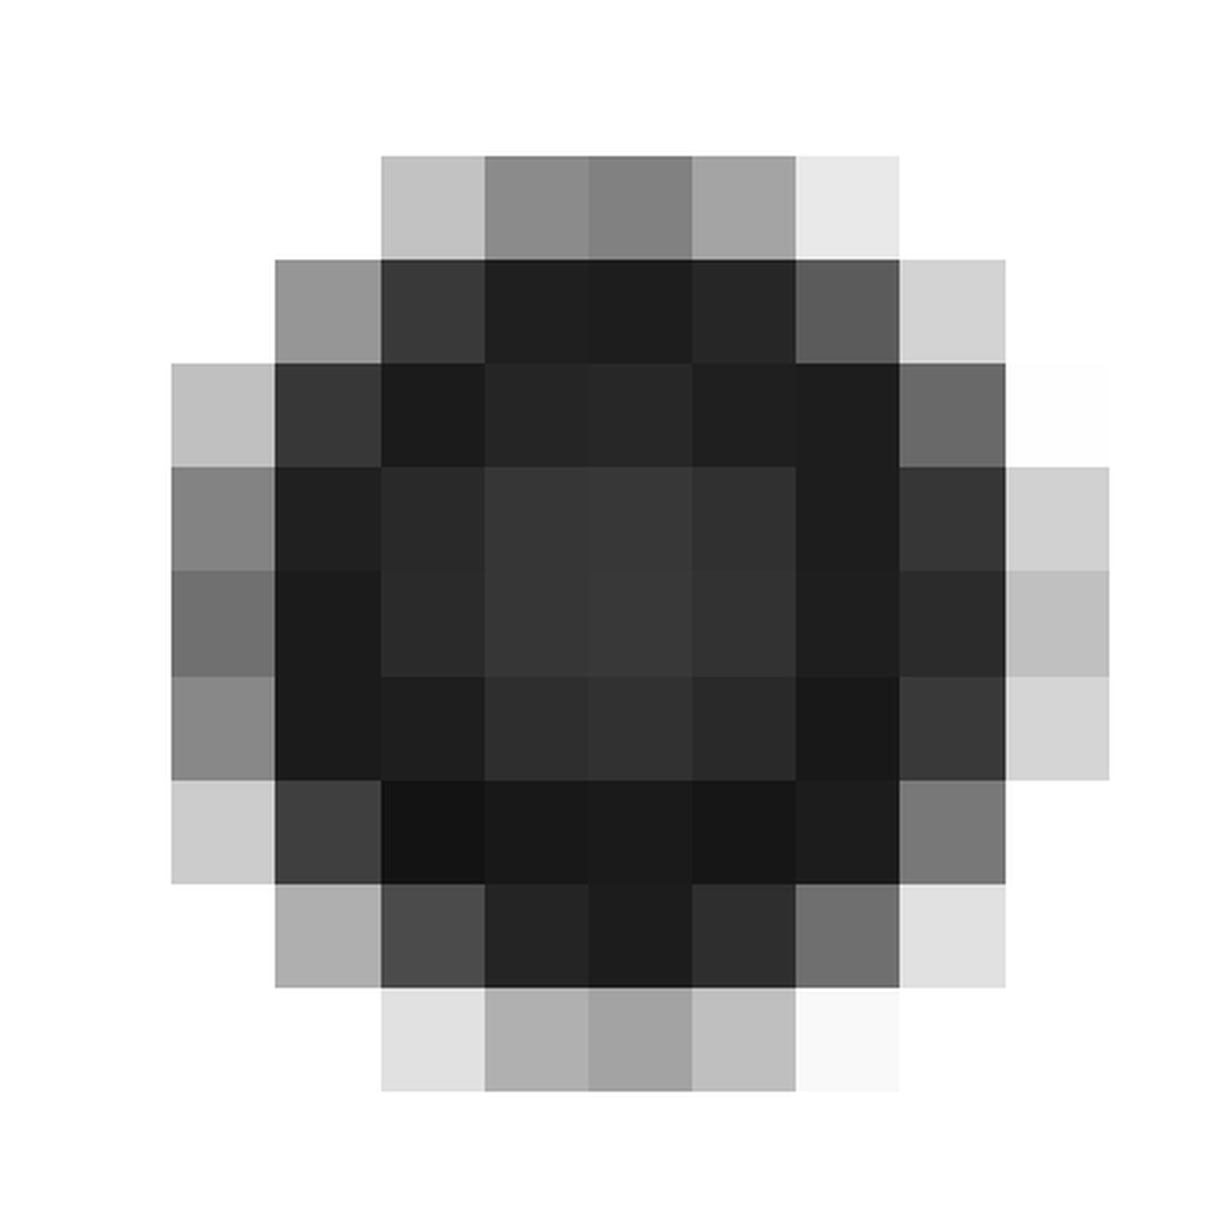
\includegraphics[scale=.11]{slicer3D/profiles/CT_x1.png}
    \caption{CT x1}
    \label{fig:CT_x1}
  \end{subfigure}
  \hfill
  \begin{subfigure}[b]{0.32\textwidth}
    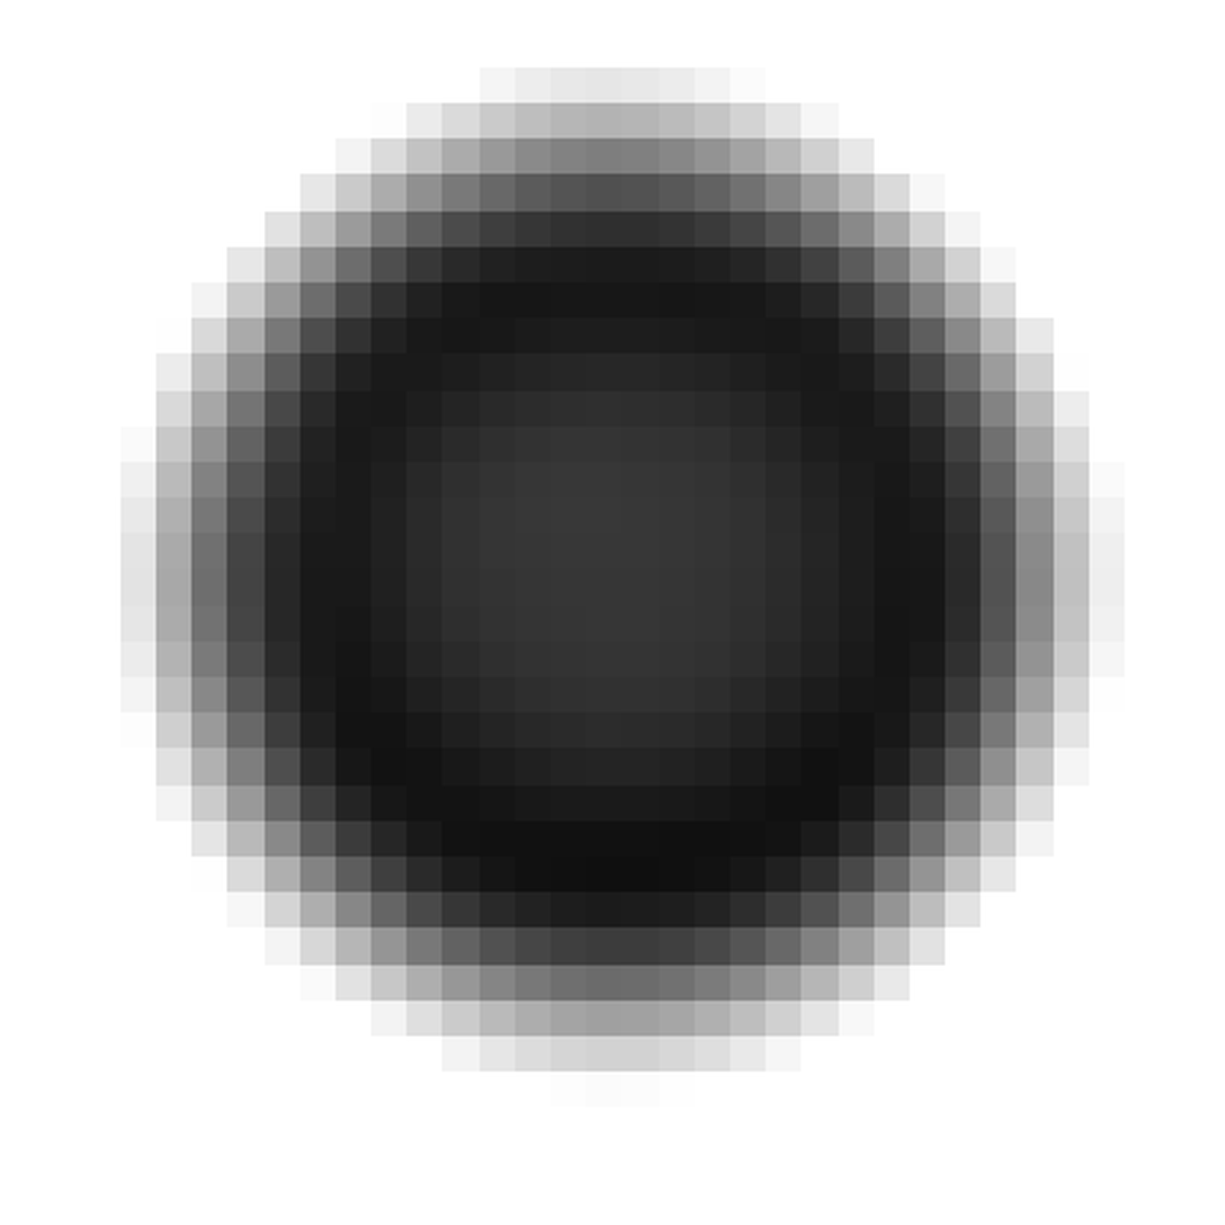
\includegraphics[scale=.11]{slicer3D/profiles/CT_x9.png}
    \caption{CT x9}
    \label{fig:CT_x9}
  \end{subfigure}
    \hfill
  \begin{subfigure}[b]{0.32\textwidth}
    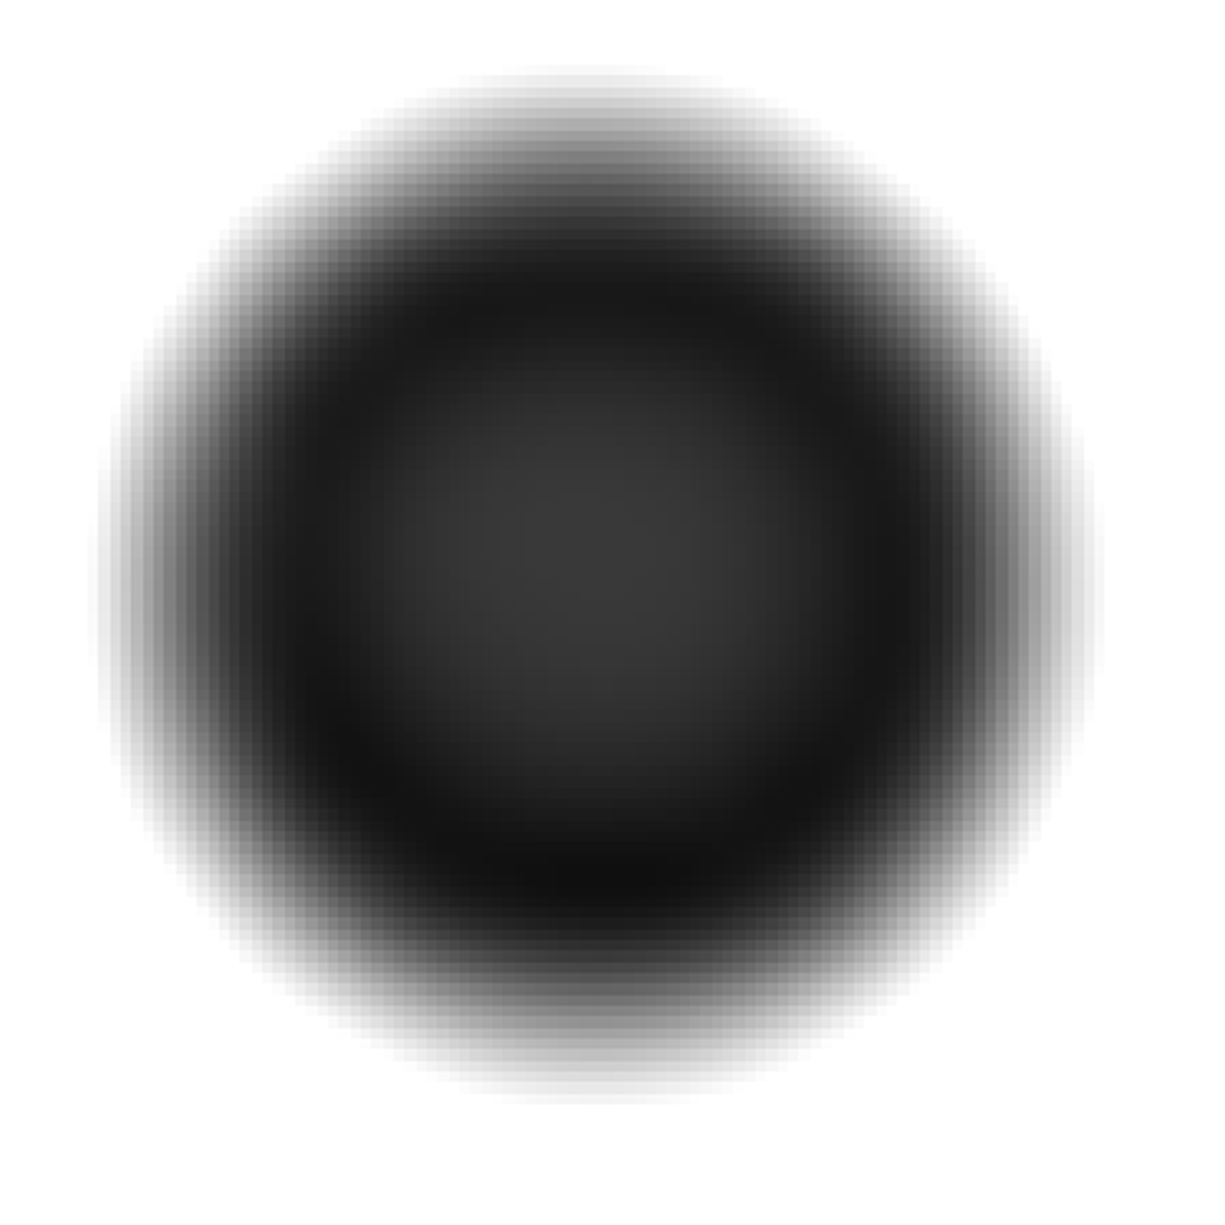
\includegraphics[scale=.11]{slicer3D/profiles/CT_x100.png}
    \caption{CT x100}
    \label{fig:CT_x100}
  \end{subfigure}
  \begin{subfigure}[b]{0.32\textwidth}
    
\includegraphics[scale=.11]{slicer3D/profiles/MR_x1.png}
    \caption{MRI x1}
    \label{fig:MRI_x1}
  \end{subfigure}
  \hfill
  \begin{subfigure}[b]{0.32\textwidth}
    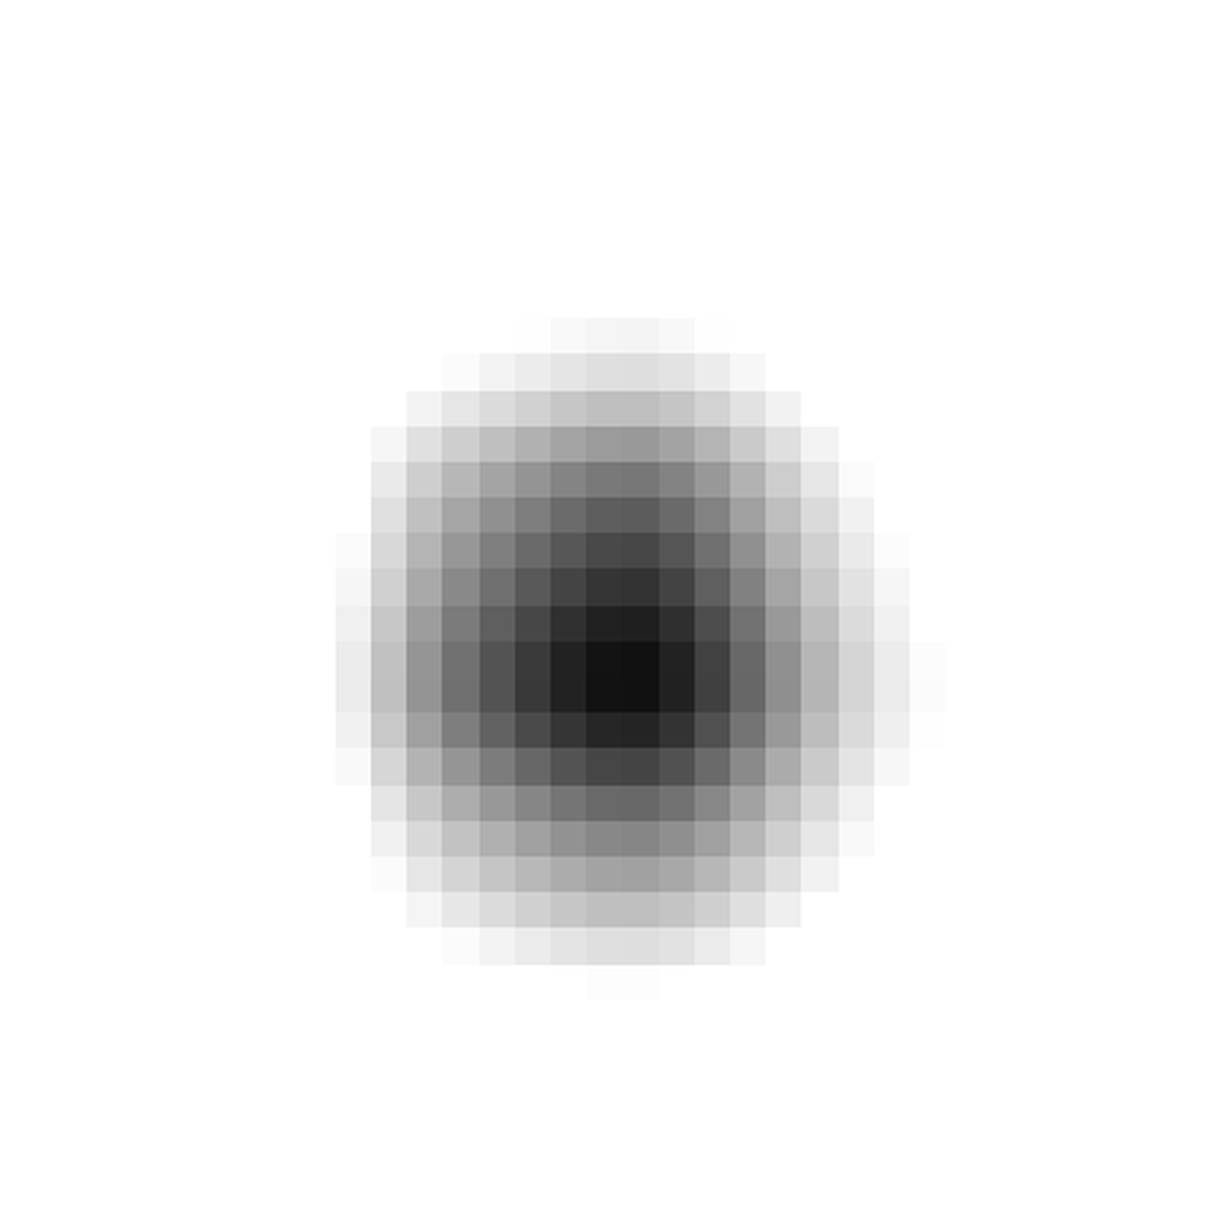
\includegraphics[scale=.11]{slicer3D/profiles/MR_x9.png}
    \caption{MRI x9}
    \label{fig:MRI_x9}
  \end{subfigure}
    \hfill
  \begin{subfigure}[b]{0.32\textwidth}
    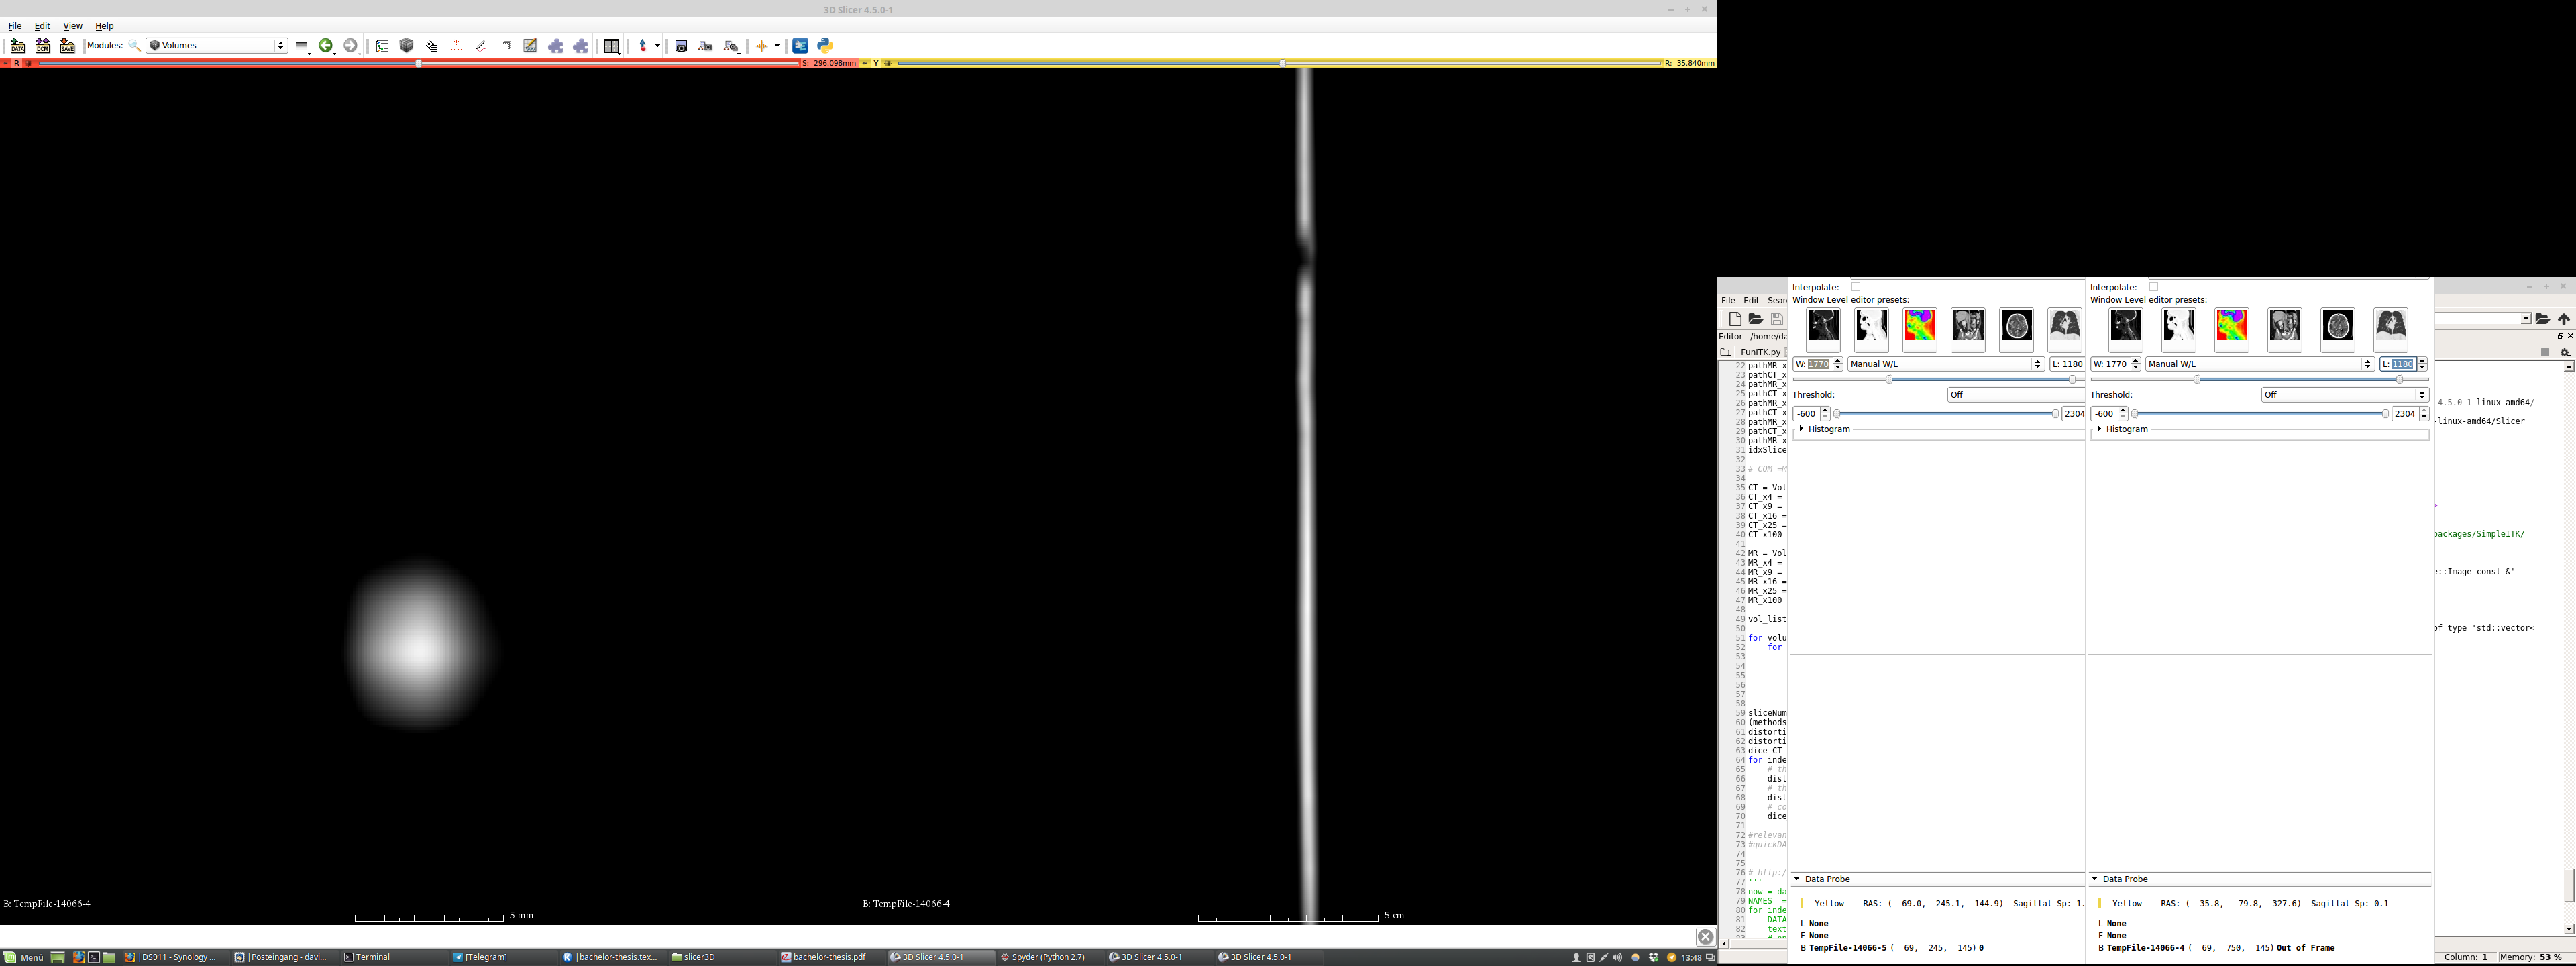
\includegraphics[scale=.11]{slicer3D/profiles/MR_x100.png}
    \caption{MRI x100}
    \label{fig:MRI_x100}
  \end{subfigure}
  \caption{CT/MRI: axial image of single rod, filling \#5  (inverted colours)}
  \label{fig:resample}
\end{figure}
\clearpage



\subsection{Capabilities}

The developed software tool is not able to automatically detect individual rods shown in a CT or MRI scan.
Instead the acquired 3D images have to be cropped to depict only a single rod.

The python script can:
\begin{itemize}
 \item denoise the image data
 \item find the brightness values of the rod, enabling it to
 \item separate pixels representing the rod from surrounding air (masking)
 \item calculate the centroid coordinates along the rod, used to
 \item calculate the local distortion
  \subitem loaction shift
  \subitem dice coefficient (roundness/deformation)
 \item plot individual rod slices
  \subitem overlaying one or two centroid coordinates
  \subitem and save it as ``.png'' file
 \item change the pixel values to reflect the distortion occuring along a rod (visualization)
 \item write the calculated numbers to a ``.txt'' file
\end{itemize}

\subsection{Measuring distortion}

Two phenomena were chosen to reflect the amount of distortion occurring in MRI scans:

\begin{enumerate}[label=\textbf{\arabic*)}]
 \item location shift (``warp'')
 \item deformation (deviation from circular profile ``DC'')
\end{enumerate}

Since the rods have a cylindrical shape, distortion can only be assessed in radial direction. To make calculations easier, the z-coordinate was put parallel to the rods, x and y radial.
Each slice (z = const.) should idealy depict the bright circular profile of the liquid (+ plastic rod in CT) surrounded by black (air).
To calculate the location shift between rods shown in CT and MRI, the coordinates of the center of mass (COM) were subtracted.
The location difference in each slice is saved as an array. Additionally, the absolute value of the coordinate shift (absCS) could be calculated.

% image of COM shift

The dice-coefficient ``DC'' (also known as Sorensen-Index) was chosen as indicator for the deviation from a circular profile. Again this value was calculated for every slice using either the CT or MRI scans.

To get a idea of the occuring distortion one should look at both the absolute value of coordinate shift and the dice-coefficient (DC).
The DC ranges from 0 to 1. A value of 1 indicates a perfect circular shape. A low DC on the other hand could be caused by many things such as:
little overlap (e.g. a ring or crescent shape); a very dark image hindering delineation of rod from background; a small circle with a radius close to a only a few pixels.


% A proposed third indicator combining warp magnitude and the DC:
% $warpDC = warpMagnitude * (1-DC)$

\subsection{Calculation: dice-coefficient (DC)}

The dice coefficient or Sorensen index \cite{MedPy_dc-doc} is defined as:

\begin{align}
DC = \frac{2 |A \, \cap \, B|}{|A| + |B|}
\end{align}

The implementation into python is based on the open source python package ``Medpy''. \cite{MedPy} A part of it's module called ``metric'' was adapted. \cite{MedPy_dc-code}
All pixels above a certain threshold will be counted as input A. The reference B is a circle whose midpoint is placed at the COM.

The caluclation of the DC is done by comparing an binary image to a circle. The position of the circle's centre and its radius is highly influencing the outcome.
Both the circle's centre and its radius were varied during the distortion assesment.


\subsection{Calculation: center of mass (COM)}

The calculation of the COM is done with help of the ``scipy'' python package.
It's module ``ndimage'' contains the function ``$center\_of\_mass()$'', which returns the COM's coordinates of a given input array.
The values assigned to voxels in CT images lie in the range from -1024 HU (air) to around 200 HU (plastic rod).
Before a meaningful result can be obtained, the values need to be shifted to be $>$ 0.
Additionally, only pixels representing the rod or the liquid should be used for the calculation.
Otherwise the almost black voxels surrounding the rod would influence the result.
This error could be observed especially if the rod is not placed in the exact middle of the scan.
As described earlier, the plastic rod is only visible in CT images. On the MRI scanns solely the liquid containded in the rods is shown. Therefore rods appear to be smaller on the MRI data.
To find the relevant pixels two algorithms were developed:

\begin{description}
 \item[1] calculating the number of pixels based on rod size
 \item[2] finding a COM resulting in good DC
\end{description}

add 1:
The inner ($4mm$) and outer ($8mm$) diameter of the rods are known. So is the \textit{pixel spacing} which respresents the equivalent size of a voxel in $mm$.
Calculating the number of pixels which make up the more or less circular profile ot the rod in each slice is calculated like this:

\begin{align}
 pixelNumber = (radius^2 \cdot \pi) \, / \, (spacing^2)
\end{align}

For CT images $radius = 4mm$, in MRI scans $radius = 2mm$. $spacing$ is the pixel spacing in x and y direction.
Next the pixels are sorted by brigthness. The top $pixelNumber$ pixels are then used to calculate the COM.

add 2:
This algorithm is a iteration method. It starts by assuming $\approx 50\%$ of all pixels in the image are part of the rod.
This first guess of $50\%$ is shifted by multiplying it with $(1 \pm 0.2) \rightarrow 1.2$ and $0.8$.
So in the first step two possible COMs are obtained using the brightest $50*1.2 = 60\%$ and $50*0.8 = 40\%$ of all pixels.
It takes note of the values assigned to the darkest and brightest pixels used during both calculations.
Those values are then set as threshold for the DC coefficient.
Effectivly it finds COM and DC for $52\%$ and $60\%$. If the DC for using 52\% is bigger, it chooses $(100\% + 50\%) / 2 = 75\%$ as next guess.
If on the other hand the DC for $40\%$ is bigger, it chooses $(0\% + 50\%) / 2 = 25\%$ as next guess.
In the second iteration it now again shifts the percentage by multiplying it with $1.2$ and $0.8$. Again COM and DC are calculated and the next guess is chosen by comparing the DCs.
This is continued until the DC value decreases compared to DC found in prior steps. The maximum DC is used as indicator for the best COM.

% image of COM shift